\chapter{Introduction}
\begin{figure}[t]
\centering
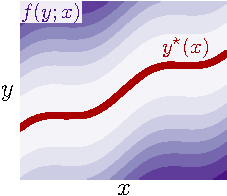
\includegraphics[width=2in]{fig/opt.pdf}
\caption{Illustration of the parametric optimization problem
  in \cref{eq:opt}.
  Each context $x$ parameterizes an
  optimization problem that the objective $f(y; x)$ depends on.
  The contours show the values of the objectives where
  darker colors indicate higher values.
  The objective is then minimized over $y$ and the resulting
  solution $y^\star(x)$ is shown in red.
  In other words, each vertical slice is an optimization problem
  and this visualization shows a continuum of optimization problems.
}
\label{fig:opt}
\end{figure}
This tutorial studies the use of machine learning
to improve repeated solves of parametric optimization
problems of the form
\begin{equation}
  y^\star(x) \in \argmin_y f(y; x),
  \label{eq:opt}
\end{equation}
where the \emph{non-convex} objective
$f: \gY\times \gX\rightarrow \R$
takes a \emph{context} or \emph{parameterization}
$x\in\gX$ which can be continuous or discrete,
and the \emph{continuous, unconstrained domain} of
the problem is $y\in\gY=\R^n$.
\Cref{eq:opt} implicitly defines a \emph{solution}
$y^\star(x)\in\gY$.
In most of the applications considered later in
\cref{sec:apps}, $y^\star(x)$ is unique and smooth,
\ie, the solution continuously changes in a
connected way as the context change s illustrated
in \cref{fig:opt}.

Parametric optimization problems such as \cref{eq:opt}
have been studied for decades
\citep{bank1982non,fiacco1990sensitivity,shapiro2003sensitivity,klatte2006nonsmooth,bonnans2013perturbation,still2018lectures,fiacco2020mathematical}
with a focus on sensitivity analysis.
The general formulation in \cref{eq:opt} captures many
tasks arising in physics, engineering, mathematics, control,
inverse modeling, and machine learning.
For example, when controlling a continuous robotic system,
$\gX$ is the space of \emph{observations} or \emph{states},
\eg, angular positions and velocities describing
the configuration of the system,
the domain $\gY\defeq \gU$ is the \emph{control space},
\eg, torques to apply to each actuated joint,
and $f(u; x)\defeq -Q(u, x)$ is the \emph{control cost}
or the negated \emph{Q-value} of the state-action tuple $(x,u)$,
\eg, to reach a goal location or to maximize the velocity.
For every encountered state $x$, the system is controlled
by solving an optimization problem in the form of \cref{eq:opt}.
While $\gY=\R^n$ is over a deterministic real-valued space
in \cref{eq:opt}, the formulation can also capture
stochastic optimization problems as discussed in
\cref{sec:extensions:sto}. For example,
\Cref{sec:apps:avi} optimizes over the (real-valued)
parameters of a variational distribution and
\cref{sec:apps:ctrl} optimizes over the (real-valued)
parameters of a stochastic policy for control and
reinforcement learning.

\begin{figure}[t]
  \centering
  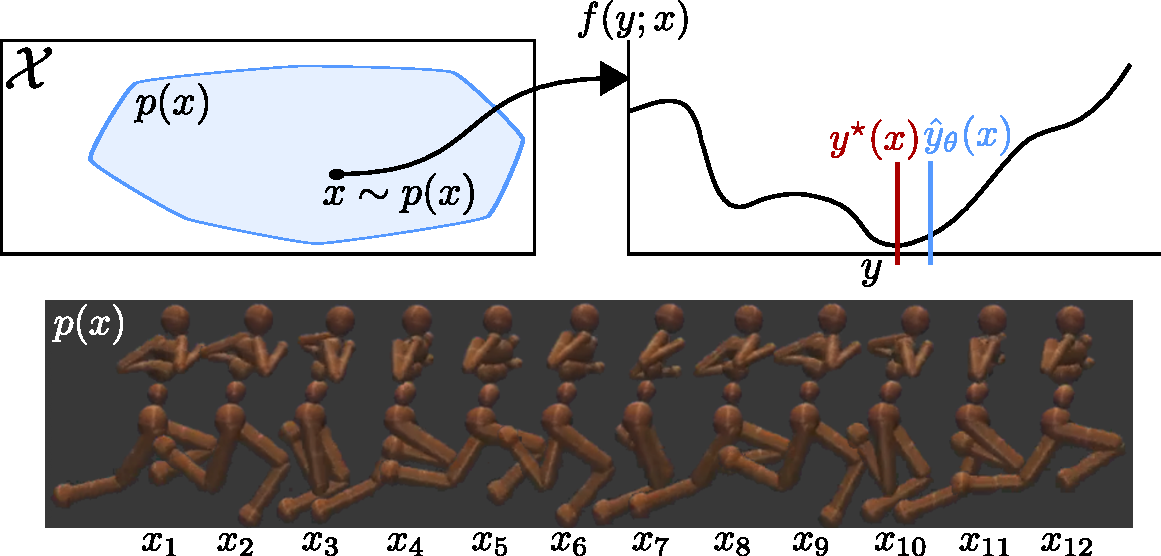
\includegraphics[width=\textwidth]{fig/overview.pdf}
  \caption{An amortized optimization method learns
    a model $\hat y_\theta$ to predict the minimum
    of an \emph{objective} $f(y;x)$ to a parameterized
    optimization problem, as in \cref{eq:opt},
    which depends on a \emph{context} $x$.
    For example, in control,
    the context space $\gX$ is the state space of the system,
    \eg angular positions and velocities describing
    the configuration of the system,
    the domain $\gY\defeq\gU$ is the control space,
    \eg torques to apply to each actuated joint,
    the cost (or negated value) of a state-action
    pair is $f(u; x)\defeq -Q(x,u)$, and the state distribution is $p(x)$.
    For an encountered state $x$,
    many reinforcement learning policies $\pi_\theta(x)\defeq\hat y_\theta(x)$
    amortize the solution to the underlying control problem
    with true solution $y^\star(x)$.
    This humanoid policy was obtained with the model-based
    stochastic value gradient in \citet{amos2021model}.
  }
  \label{fig:overview}
\end{figure}


Optimization problems such as \cref{eq:opt} quickly become a
computational bottleneck in systems they are a part of.
These problems often does not have a closed-form
analytic solution and is instead solved with
approximate numerical methods which iteratively
search for the solution.
This computational problem has led to many specialized
solvers that leverage domain-specific insights to
deliver fast solves.
Specialized algorithms are
especially prevalent in convex optimization methods for
linear programming, quadratic programming, cone programming,
and control and use theoretical insights of the problem
structure to bring empirical gains of computational
improvements and improved convergence
\citep{boyd2004convex,nocedal2006numerical,bertsekas2015convex,bubeck2015convex,nesterov2018lectures}.

Mostly separate from optimization research and algorithmic advancements,
the machine learning community has focused on developing
generic function approximation methods for estimating non-trivial
high-dimensional mappings from data
\citep{murphy2012machine,goodfellow2016deep,deisenroth2020mathematics}.
While machine learning models are often used to reconstruct mappings
from data, \eg for supervised classification or regression where
the targets are given by human annotations.
Many computational advancements on the software and hardware
have been developed in recent years to make the prediction time fast:
the forward pass of a neural network generating a prediction
can execute in milliseconds on a graphics processing unit.

\textbf{Overview.}
This tutorial studies the use of machine learning models to
rapidly predict the solutions to the optimization problem in
\cref{eq:opt}, which is referred to as
\emph{amortized optimization} or \emph{learning to optimize}.
Amortized optimization methods are capable of significantly
improving the computational time of
classical algorithms \emph{on a focused subset of problems}.
This is because the model is able to learn about the
solution mapping from $x$ to $y^\star(x)$ that classical
optimization methods usually do not assume access to.
My goal in writing this is to explore a unified perspective
of modeling approaches of amortized optimization in
\cref{sec:foundations} to help draw connections
between the applications in \cref{sec:apps},
\eg between amortized variational inference, meta-learning,
and policy learning for control and reinforcement learning,
sparse coding, convex optimization, optimal transport,
and deep equilibrium networks.
These topics have historically been studied in isolation
without connections between their amortization components.
\Cref{sec:implementation} presents a computational tour
through source code for variational inference, policy learning,
and a spherical optimization problem and
\cref{sec:discussion} concludes with a discussion of
challenges, limitations, open problems, and related work.

\textbf{How much does amortization help?}
Amortized optimization has been revolutionary to many fields,
especially including variational inference and reinforcement
learning.
\Cref{fig:vae-performance} shows that the amortization component
of a variational autoencoder trained on MNIST is \textbf{25000}
times faster (0.4ms vs.~8 seconds!) than solving a batch of
1024 optimization problems from scratch to obtain a
solution of the same quality.
These optimization problems are solved in every training iteration
and can become a significant bottleneck if they are
inefficiently solved.
If the model is being trained for millions of iterations,
then the difference between solving the optimization problem
in 0.4ms vs.~8 seconds makes the difference between the
entire training process finishing in a few hours or a month.

\textbf{A historic note: amortization in control and statistical inference.}
Amortized optimization has arisen in many fields as a result
to practical optimization problems being non-convex and not
having easily computed, or closed-form solutions.
Continuous control problems with linear dynamics and quadratic
cost are convex and often easily solved with the linear
quadratic regulator (LQR) and many non-convex extensions and
iterative applications of LQR have been successful over
the decades, but becomes increasingly infeasible on
non-trivial systems and in reinforcement learning settings
where the policy often needs to be rapidly executed.
For this reason, the reinforcement learning community almost
exclusively amortizes control optimization problems with
a learned policy \citep{sutton2018reinforcement}.
Related to this throughline in control and reinforcement learning,
many statistical optimization problems have closed
form solutions for known distributions such as Gaussians.
For example, the original Kalman filter is defined with Gaussians
and the updates take closed-form. The extended Kalman filter
generalizes the distributions to non-Gaussians, but the updates
are in general no longer available analytically and need to be
computationally estimated.
\citet{marino2018general} shows how amortization helps improve
this computationally challenging step.
Both of these control and statistical settings start with a
simple setting with analytic solutions to optimization problems,
generalize to more challenging optimization problems
that need to be computationally estimated, and then
add back some computational tractability with amortized optimization.


%%% Local Variables:
%%% coding: utf-8
%%% mode: latex
%%% TeX-master: "../amor-nowplain.tex"
%%% LaTeX-biblatex-use-Biber: True
%%% End: